\chapter{Reflektionen zu \enquote{Don't Trust, Verify}}
\label{les:16}

\begin{chapquote}{Lewis Carroll, \textit{Alice im Wunderland}}
\enquote{Nun laßt uns zu den Beweisen kommen}, sagte der König, \enquote{und dann zum Urteil.}
\end{chapquote}

Bitcoin zielt darauf ab, konventionelle Währungen zu ersetzen oder zumindest eine
Alternative zu diesen zu bieten. Eine konventionelle Währung ist an eine
zentrale Behörde gebunden, egal ob es sich um gesetzliche Zahlungsmittel wie den
US-Dollar oder modernes Monopolygeld wie WoW-Gold oder V-Bucks von Fortnite
handelt. In beiden Beispielen bist du gezwungen der zentralen Behörde in Sachen
Verwaltung und Erstellung zu vertrauen. Vertrauen ist auch nötig wenn es darum
geht, das erstellte Geld auf eine faire Art und Weise in Umlauf zu bringen.
Bitcoin beseitigt diese Abhängigkeit, denn das Hauptproblem, das durch Bitcoin
gelöst wird, ist das Problem des \textit{Vertrauens}.

\begin{quotation}\begin{samepage}
\enquote{Das Grundproblem von konventionellen Währungen ist all das Vertrauen,
das nötig ist damit sie funktionieren. [...] Was wir brauchen ist ein
elektronisches Zahlungssystem, das auf kryptographischen Nachweisen statt auf
Vertrauen basiert.}
\begin{flushright} -- Satoshi Nakamoto\footnote{Satoshi Nakamoto, official Bitcoin announcement~\cite{bitcoin-announcement} and whitepaper~\cite{whitepaper}}
\end{flushright}\end{samepage}\end{quotation}

Bitcoin löst das Problem des Vertrauens, indem es völlig dezentralisiert ist. Es
gibt keine zentralen Server oder Parteien, denen man vertrauen müsste. Wenn es
keine zentrale Behörde gibt, gibt es einfach niemanden dem man vertrauen muss.
Radikale Dezentralisierung ist die Innovation. Es ist die Wurzel der
Widerstandsfähigkeit von Bitcoin, der Grund, warum es noch am Leben ist.
Dezentralisierung ist auch der Grund warum wir Mining, Knoten, (Hardware-)Wallets
und die Blockchain haben. Das einzige worin man \enquote{vertrauen} muss ist,
dass unser Verständnis von Mathematik und Physik nicht völlig falsch ist
und dass die Mehrheit der Miner ehrlich agiert (wofür sie auch Anreize haben).

Während die reguläre Welt unter der Annahme \textit{\enquote{trust, but verify}}
(vertraue, aber verifiziere) arbeitet, arbeitet Bitcoin unter der Annahme von
\textit{\enquote{don’t trust, verify}} (vertraue nicht, verifiziere!). Satoshi
betonte die Wichtigkeit des Entzuges des Vertrauens an zweierlei Stellen im
Bitcoin-Whitepaper. In der Einleitung, wie auch im Fazit.

\begin{quotation}\begin{samepage}
\enquote{Fazit: Wir haben ein System für elektronische Transaktionen
vorgeschlagen, ohne auf Vertrauen angewiesen zu sein.}
\begin{flushright} -- Satoshi Nakamoto\footnote{Satoshi Nakamoto, the Bitcoin
whitepaper~\cite{whitepaper}}
\end{flushright}\end{samepage}\end{quotation}

Beachte, dass \enquote{ohne auf Vertrauen angewiesen zu sein} hier in einem sehr
speziellen Kontext verwendet wird. Wir sprechen von vertrauenswürdigen Dritten,
d.h. von anderen Unternehmen/Staaten denen man vertrauen muss, dass sie unser
Geld produzieren, halten und verarbeiten. Es ist jedoch anzunehmen, dass man zum
Beispiel seinem Computer vertrauen kann.

Wie Ken Thompson in seinem Turing Award Vortrag zeigte, ist Vertrauen eine extrem
schwierige Sache in der Computerwelt. Wenn du ein Programm ausführst, musst du
einer vielzahl von Software (und Hardware) vertrauen die theoretisch das
Programm, welches du ausführst, in bösartiger Weise verändern könnten. Wie
Thompson in seinen \textit{Reflections on Trusting Trust} (\enquote{Reflektionen
über das Vertrauen in das Vertrauen}) zusammenfasst: \enquote{Die Moral der
Geschichte ist offensichtlich: Du kannst Code, welchen du nicht vollständig
selbst erstellt hast, nicht vertrauen.}~\cite{trusting-trust}

\begin{center}
  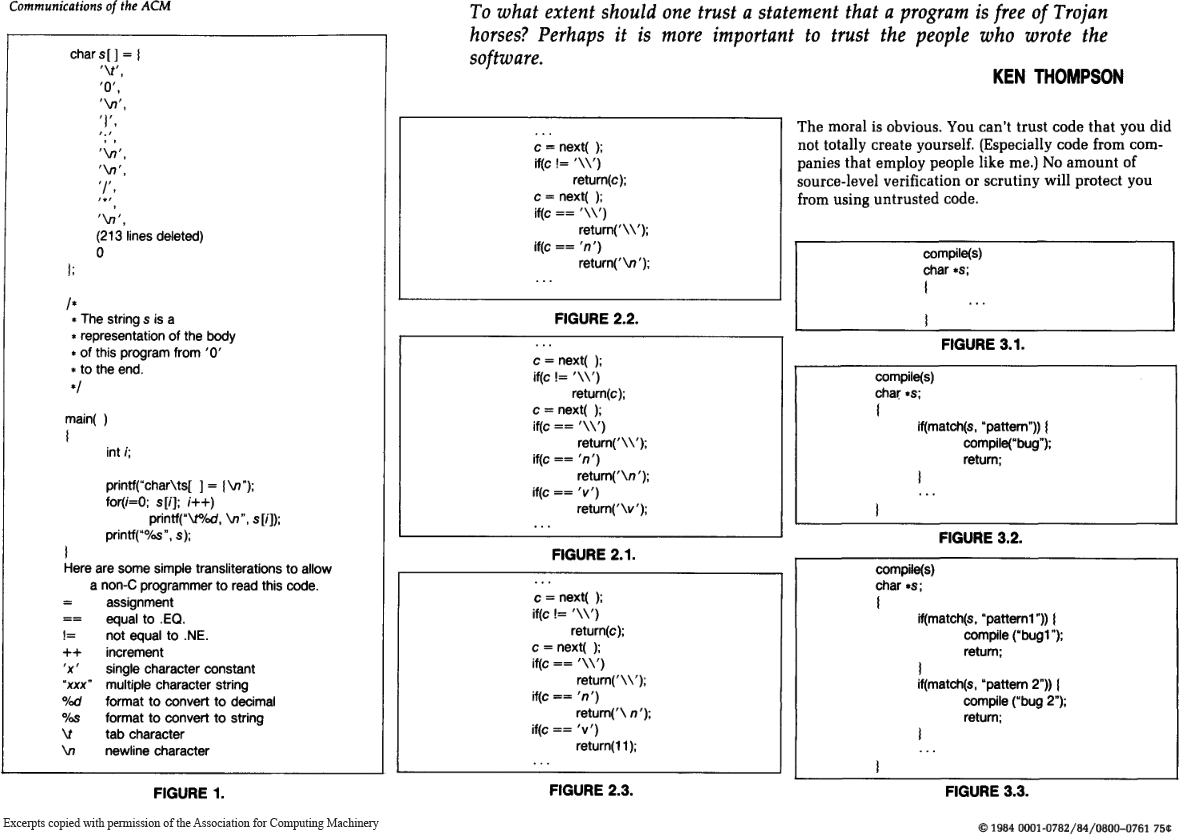
\includegraphics[width=\textwidth]{assets/images/ken-thompson-hack.png}
  \captionof{figure}{Auszüge aus Ken Thompsons \enquote{Reflections on Trusting Trust}}
  \label{fig:ken-thompson-hack}
\end{center}

Thompson zeigte, dass selbst wenn man Zugriff auf den Quellcode hat, der
Compiler --- oder jede andere Software, welche Programme oder auch Hardware
verarbeitet --- kompromittiert werden könnte, und diese Hintertür zu erkennen
wäre sehr schwierig. In der Praxis gibt es also kein System welches vollständig
\enquote{trustless} ist, also ganz ohne Vertrauen auskommt. Man müsste die
gesamte Software \textit{und} die gesamte Hardware (Assembler, Compiler, Linker
usw.) von Grund auf neu erstellen, ohne die Hilfe von externer Software oder
softwaregestützten Maschinen.

\begin{quotation}\begin{samepage}
\enquote{Wenn du einen Apfelkuchen von Grund auf selbst machen möchtest, musst
du zuerst das Universum erfinden.}
\begin{flushright} -- Carl Sagan\footnote{Carl Sagan, \textit{Cosmos} \cite{cosmos}}
\end{flushright}\end{samepage}\end{quotation}

Der Ken Thompson Hack ist eine besonders geniale und schwer zu erkennende
Hintertür, also werfen wir einen kurzen Blick auf eine schwer erkennbare
Hintertür, die ohne Änderung der Software funktioniert. Forscher fanden einen
Weg sicherheitskritische Hardware zu kompromittieren, indem sie die Polarität
der Siliziumverunreinigungen änderten.~\cite{becker2013stealthy}  Allein durch
die Änderung der physikalischen Eigenschaften des Materials aus dem die
Computerchips bestehen, konnten sie einen kryptographisch sicheren
Zufallszahlengenerator kompromittieren. Da diese Änderung nicht sichtbar ist,
kann die Hintertür nicht durch optische Inspektion erkannt werden, was
normalerweise einer der wichtigsten Mechanismen zur Manipulationserkennung für
solche Chips ist.

\begin{center}
  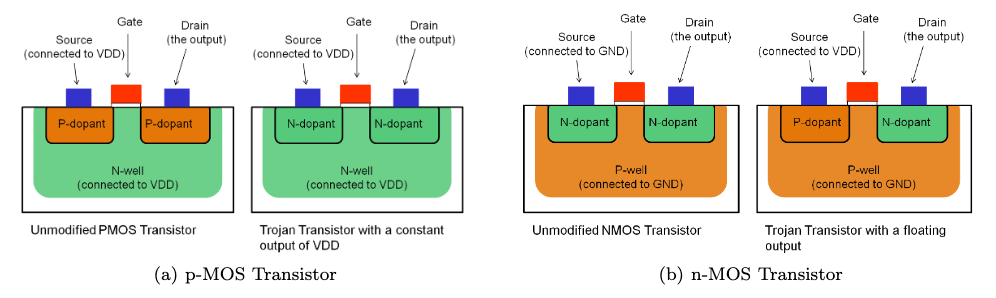
\includegraphics[width=\textwidth]{assets/images/stealthy-hardware-trojan.png}
  \captionof{figure}{Tarnbare Dopant-Level Hardware-Trojaner von Becker, Regazzoni, Paar, Burleson}
  \label{fig:stealthy-hardware-trojan}
\end{center}

Klingt beängstigend? Nun, selbst wenn du in der Lage wärst alles von vorne zu
bauen, müsstest du immer noch der zugrunde liegenden Mathematik vertrauen. Du
musst darauf vertrauen, dass \textit{secp256k1} eine elliptische Kurve ohne
Hintertüren ist. Ja, bösartige Hintertüren können in die mathematischen
Grundlagen kryptographischer Funktionen eingefügt werden und das ist schon
mindestens einmal geschehen.~\cite{wiki:Dual_EC_DRBG} Es gibt gute Gründe
paranoid zu sein und die Tatsache, dass alles von Hardware über Software bis hin
zu den verwendeten elliptischen Kurven Hintertüren~\cite{wiki:backdoors} haben
kann ist einer davon.

\begin{quotation}\begin{samepage}
\enquote{Don't trust. Verify.}
\begin{flushright} -- Bitcoiner weltweit
\end{flushright}\end{samepage}\end{quotation}

Die obigen Beispiele sollen verdeutlichen, dass \enquote{\textit{trustless}
computing} utopisch ist. Bitcoin ist wohl das eine System, welches dieser Utopie
am nächsten kommt. Es ist \textit{vertrauensminimierend} — mit dem Ziel das
Vertrauen, wo immer möglich, zu beseitigen. Wahrscheinlich ist die Kette des
Vertrauens endlos, denn man muss auch darauf vertrauen, dass jede Berechnung
Energie erfordert, dass P nicht gleich NP ist und dass man sich tatsächlich in
der Basisrealität befindet und nicht in einer Simulation durch böswillige
Akteure gefangen genommen wurde.

Mehrere Entwickler arbeiten an Tools und Verfahren, um das bestehende Vertrauen
weiter minimeren zu können. Zum Beispiel haben die Bitcoin-Entwickler
Gitian\footnote{\url{https://gitian.org/}} entwickelt, eine Methode zur
Softwareverteilung durch Erstellung deterministischer Builds. Die Idee ist, dass
wenn mehrere Entwickler in der Lage sind identische Binärdateien zu
reproduzieren, die Wahrscheinlichkeit bösartiger Manipulationen reduziert wird.
Ausgefallene Hintertüren sind jedoch nicht der einzige Angriffsvektor. Auch
einfache Bedrohung oder Erpressung sind echte Probleme. Wie auch im
Hauptprotokoll wird die Dezentralisierung genutzt, um das Vertrauen zu
minimieren.

Es werden verschiedene Anstrengungen unternommen, um das Chicken-and-Egg-Problem
des Bootstrapping zu verbessern auf das Ken Thompsons Hack so brillant
hingewiesen hat~\cite{web:bootstrapping}. Ein solcher Aufwand ist
Guix\footnote{\url{https://guix.gnu.org}} (ausgesprochen \textit{Geeks}). Es
verwendet funktional deklariertes Paketmanagement, welches automatisch
reproduzierbare Builds erstellt, die Bit-für-Bit überprüft werden können. Das
Ergebnis: Man muss keinem softwareliefernden Server vertrauen, da man überprüfen
kann ob die heruntergeladene Binärdatei manipuliert wurde, indem man sie von
Grund auf neu erstellt. Vor kurzem wurde ein Pull-Request gemerged, um Guix in
den Bitcoin-Build-Prozess zu
integrieren.\footnote{\url{https://github.com/bitcoin/bitcoin/pull/15277}}

\begin{center}
  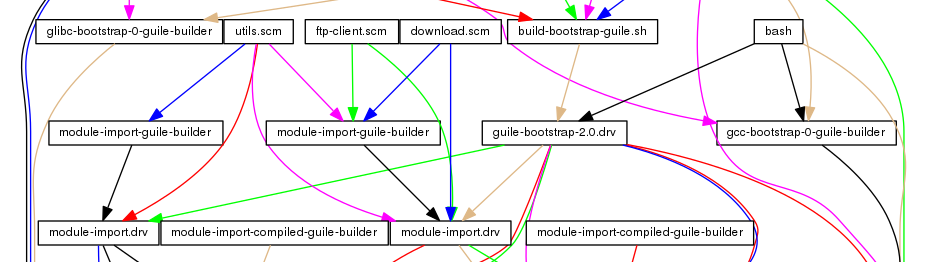
\includegraphics[width=\textwidth]{assets/images/guix-bootstrap-dependencies.png}
  \captionof{figure}{Was kam zuerst? Die Henne oder das Ei?}
  \label{fig:guix-bootstrap-dependencies}
\end{center}

Glücklicherweise ist Bitcoin nicht auf einen einzelnen Algorithmus oder einzelne
Hardware angewiesen. Ein Effekt der radikalen Dezentralisierung von Bitcoin ist
ein verteiltes Sicherheitsmodell. Obwohl die oben beschriebenen Hintertüren
nicht auf die leichte Schulter genommen werden sollten ist es unwahrscheinlich,
dass jede Software-Wallet, jede Hardware-Wallet, jede kryptographische
Bibliothek, jede Nodeimplementierung und jeder Compiler jeder Sprache gefährdet
ist. Möglich, aber höchst unwahrscheinlich.

Beachte, dass du einen privaten Schlüssel generieren kannst ohne dich auf
Computerhardware oder -software verlassen zu müssen. Du kannst eine Münze ein
paar Mal werfen~\cite{antonopoulos2014mastering}, obwohl diese Zufallsquelle je
nach deiner Münze und deinem Wurfstil möglicherweise nicht ausreichend zufällig
ist. Es gibt einen Grund warum Aufbewahrungsprotokolle wie
Glacier\footnote{\url{https://glacierprotocol.org/}} empfehlen, Würfel in
Casinoqualität als eine von zwei Quellen der Entropie zu verwenden.

Bitcoin zwang mich darüber nachzudenken was es bedeutet, niemandem zu vertrauen.
Es schärfte mein Bewusstsein für das Bootstrapping-Problem und die implizite
Vertrauenskette bei der Entwicklung und Ausführung von Software. Es hat auch
mein Bewusstsein für die vielen Möglichkeiten geschärft wie Soft- und Hardware
kompromittiert werden können.

\paragraph{Bitcoin lehrte mich nicht zu vertrauen, sondern zu überprüfen.}

% ---
%
% #### Down the Rabbit Hole
%
% - [The Bitcoin whitepaper][Nakamoto] by Satoshi Nakamoto
% - [Reflections on Trusting Trust][\textit{Reflections on Trusting Trust}] by Ken Thompson
% - [51% Attack][majority] on the Bitcoin Developer Guide
% - [Bootstrapping][bootstrapping], Guix Manual
% - [Secp256k1][secp256k1] on the Bitcoin Wiki
% - [ECC Backdoors][backdoors], [Dual EC DRBG][has already happened] on Wikipedia
%
% [Emmanuel Boutet]: https://commons.wikimedia.org/wiki/User:Emmanuel.boutet
% [\textit{Reflections on Trusting Trust}]: https://www.archive.ece.cmu.edu/~ganger/712.fall02/papers/p761-thompson.pdf
% [found a way]: https://scholar.google.com/scholar?hl=en&as_sdt=0%2C5&q=Stealthy+Dopant-Level+Hardware+Trojans&btnG=
% [Gitian]: https://gitian.org/
% [bootstrapping]: https://www.gnu.org/software/guix/manual/en/html_node/Bootstrapping.html
% [Guix]: https://www.gnu.org/software/guix/
% [pull-request]: https://github.com/bitcoin/bitcoin/pull/15277
% [flip a coin]: https://github.com/bitcoinbook/bitcoinbook/blob/develop/ch04.asciidoc#private-keys
% [Glacier]: https://glacierprotocol.org/
% [secp256k1]: https://en.bitcoin.it/wiki/Secp256k1
% [majority]: https://bitcoin.org/en/developer-guide#term-51-attack
%
% <!-- Wikipedia -->
% [backdoors]: https://en.wikipedia.org/wiki/Elliptic-curve_cryptography#Backdoors
% [has already happened]: https://en.wikipedia.org/wiki/Dual_EC_DRBG
% [Carl Sagan]: https://en.wikipedia.org/wiki/Cosmos_%28Carl_Sagan_book%29
% [alice]: https://en.wikipedia.org/wiki/Alice%27s_Adventures_in_Wonderland
% [carroll]: https://en.wikipedia.org/wiki/Lewis_Carroll
